\chapter{Proposed Work: Design-time Timing Analysis of Component-based Distributed Real-time Embedded Systems}

\section{Colored Petri net-based Modeling and Analysis Methodology}

% Describe DREMS
\subsection{Design Model: Distributed Managed Systems (DREMS)}

The target component model and architecture used to illustrate the proposed timing analysis methods is the DREMS infrastructure (\iapfull) \cite{DREMS13Software}, \cite{ISIS_F6_ISORC:13}. DREMS was designed and implemented for a class of distributed real-time embedded systems that are remotely deployed and are characterized by strict timing requirements e.g. a cluster of satellites. DREMS is a software infrastructure for the design, implementation, deployment and management of component-based real-time embedded systems. The infrastructure includes design-time modeling tools \cite{ISIS_F6_SFFMT:13} that integrate with a well-defined and fully implemented component model \cite{ISIS_F6_ISORC:13, kumar2014colored} used to build component-based applications. Rapid prototyping and code generation features coupled with a modular runtime platform automate the tedious aspects of the software development and enable robust deployment and operation of mixed-criticality distributed applications.

The DREMS component model is based on the Component Integrated ACE ORB (CIAO) \cite{RT_CIAO:04, CIAO_Chap:04} project. CIAO is an implementation of the OMG's Lightweight CORBA Component Model (CCM) \cite{CCM-light:03}. CIAO uses the
TAO~\cite{TAO:02} CORBA object request broker (ORB) as its default underlying
communication middleware.  With the recent standardization of connector mechanisms~\cite{dds4ccm:09}, CIAO is also able to support asynchronous messaging and the OMG Data Distribution Service (DDS) through its ports. Unlike CIAO, the DREMS component model is not tightly coupled with the CORBA transport mechanisms. All component communication is via ports and connectors \cite{Connectors} enabling a variety of interaction schemes. For safe and deadlock-free behavior, this component model also allows only one thread of control per component to be active at any given instant of time. 

\begin{figure}[h]
	\centering
	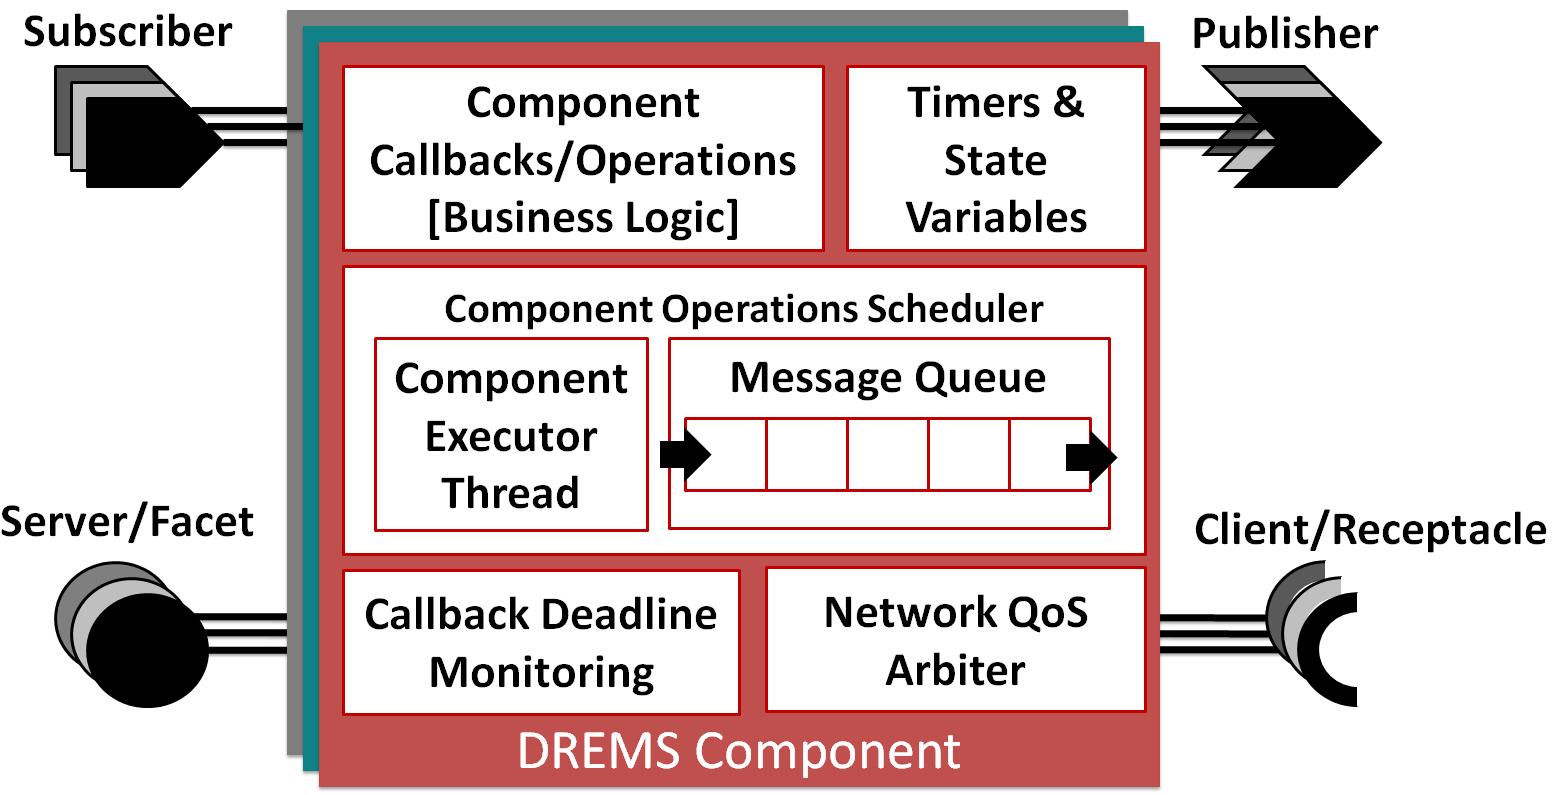
\includegraphics[width=\textwidth]{./figs/drems_component}
	\caption{DREMS Component}
	\label{fig:DREMS_Component}
	\vspace{-0.1in}
\end{figure}


Figure \ref{fig:DREMS_Component} presents a typical DREMS-style component. Component-based software engineering relies on the principle of assembly: Large and complicated systems can be iteratively constructed by composing small reusable component building blocks. Each \emph{component} contains a set of communication ports and interfaces, a message queue, time-triggered event handling and state variables. Using ports, components communicate with the external world. Using interfaces and message passing schemes, components process requests from other components. This interaction mechanism lies at the heart of component-based software. 

Each DREMS component supports four basic types of ports for interaction with other collaborating components: Facets, Receptacles, Publishers and Subscribers. A component's {\bf facet} is a unique interface that it exposes to its clients. This interface can be invoked either synchronously via remote method invocation (RMI) or asynchronously via asynchronous method invocation (AMI) \cite{waldo1998remote, raje1997asynchronous}. A component's {\bf receptacle} specifies an interface required by the component in order to function correctly. Using its receptacle, a component can establish connections and invoke operations on other components using either RMI or AMI. A {\bf publisher} port is a single point of data emission. This port emits data produced by a component operation. A {\bf subscriber} port is a single point of data consumption, feeding received data to the associated component. Communication between publishers and subscribers is contingent on the compatibility of their associated topics. Publishers and Subscribers enable the OMG DDS anonymous publish/subscribe \cite{eugster2003many} style of messaging. More details on this component model can be found in ~\cite{ISIS_F6_ISORC:13}.

\subsubsection{Component Operations}

An operation is an abstraction for the different tasks undertaken by a component. These tasks are implemented by the component's executor code written by the developer. Application developers provide the functional, \emph{business-logic} code that implements operations on the state variables e.g. a PID control operation could receive the current state of dynamic variables from a \emph{Sensor} Component, and using the relevant gains calculate a new state to which an \emph{Actuator} component should progress the system. In order to service interactions with the underlying framework and with other components, every component is associated with a message queue. This queue holds instances of operations ('messages') that are ready for execution and need to be serviced by the component. These operations service either interaction requests (seen on communication ports) or service requests (from the underlying framework). An example for the latter is the use of component timers that can periodically (or sporadically) activate an operation. 

Figure \ref{fig:component_operations} shows the basic structure of this model. Each operation is characterized by a priority and a deadline. Operation deadlines are quantified in absolute time measured starting from when the operation is enqueued onto the component message queue. These operations are sorted and scheduled based on one of three scheduling schemes: Earliest Deadline First (EDF), First In First Out (FIFO), or Priority FIFO (PFIFO). 

\begin{figure}[ht]
	\centering
	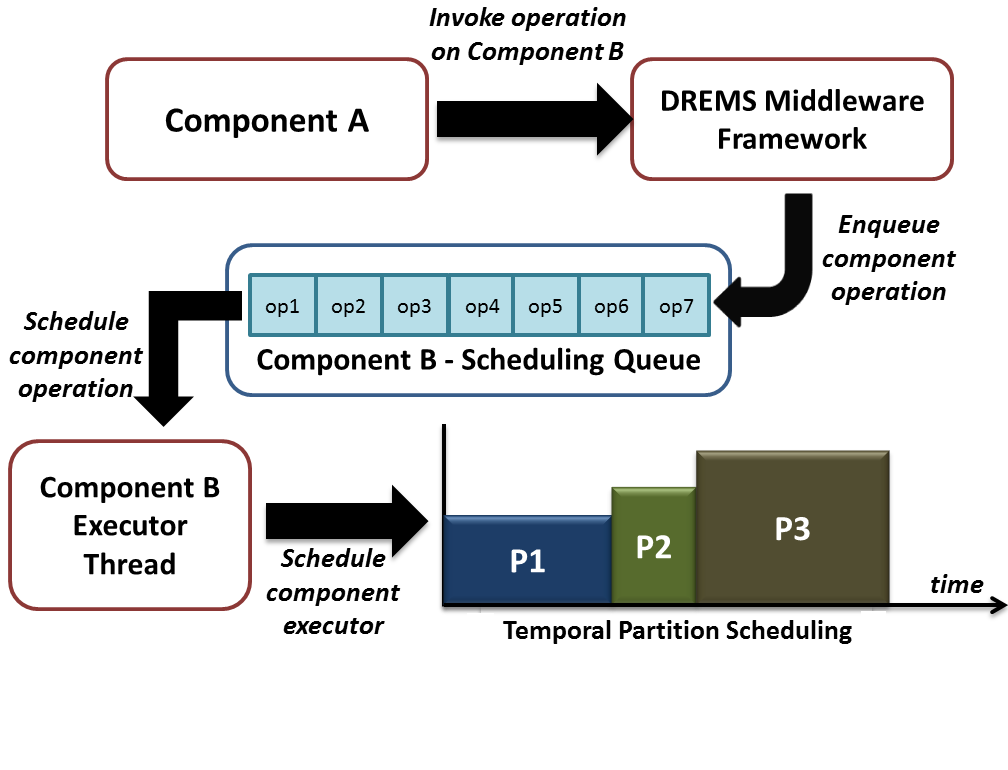
\includegraphics[width=\textwidth]{./figs/component_operations}
	\caption{Scheduling Component Operations}
	\label{fig:component_operations}
\end{figure}
%\vspace{0.2in}

To facilitate component behavior that is free of deadlocks and race conditions, the component's execution is handled on a single thread. Operations in the message queue are therefore scheduled one at a time under a non-preemptive policy. A component dispatcher thread dequeues the next ready operation from the component message queue. This operation is scheduled for execution on a component executor thread. The operation is run to completion before another operation from the queue is serviced. This single-threaded execution helps avoid synchronization primitives such as internal state variables that lead to strenuous code development. Though components that share a processor still run concurrently, each component operation is executed on a single component-specific executor thread.

Figure \ref{fig:timing_diagram} shows a sample timing diagram of how a component operation is handled. At time 0, the component executor thread is running some previously ready component operation, \emph{op1}. At this point, consider that a new component operation \emph{op2} is enqueued onto the message queue and marked as ready. At time 10, assuming that no other component requires scheduling, the component dispatcher thread of this component dequeues the next ready operation for execution. Assuming the component executor thread is scheduled immediately by the underlying processor, this thread runs the ready operation by invoking its \emph{execute} function. This operation is run to completion at time 16. The total time taken for execution of this operation is measured from when the operation was enqueued, i.e. time 0. If the time taken for the operation exceeds its deadline, a fault manager is immediately notified. The duration of the component operation is further delayed by temporal partitioning enforced by the OS scheduler. This adds to the need for schedulability analysis, especially in case of safety and mission-critical applications.

\begin{figure}[ht]
	\centering
	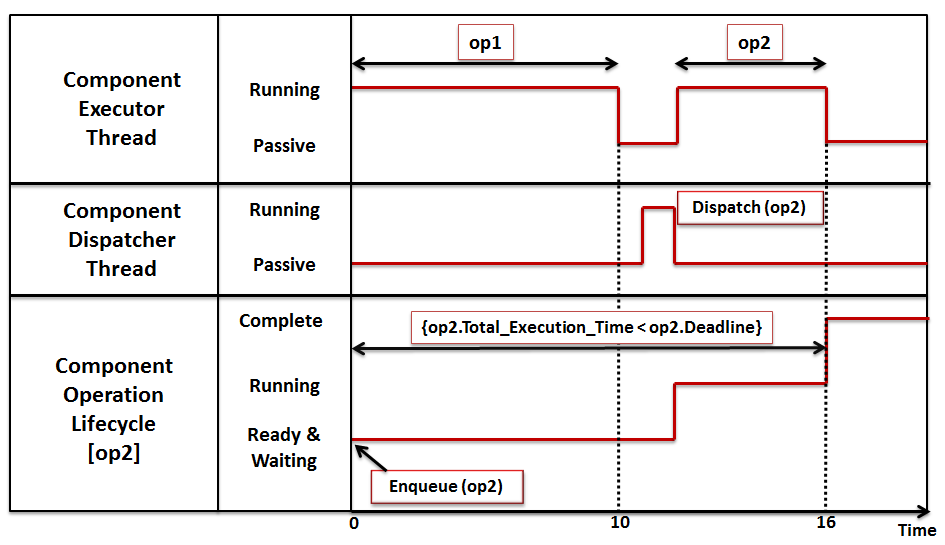
\includegraphics[width=\textwidth]{./figs/cop_timing_diagram}
	\caption{Component Operation Execution}
	\label{fig:timing_diagram}
\end{figure}

\subsubsection{Temporal Partition Scheduler}

DREMS components are grouped into processes that are assigned to temporal partitions, implemented by the DREMS OS scheduler. This scheduler was implemented by modifying the behavior of the standard Linux scheduler, introducing an ARINC-653 ~\cite{ARINC-653} style temporal and spatial partitioning scheme. 

\begin{figure}[ht]
	\centering
	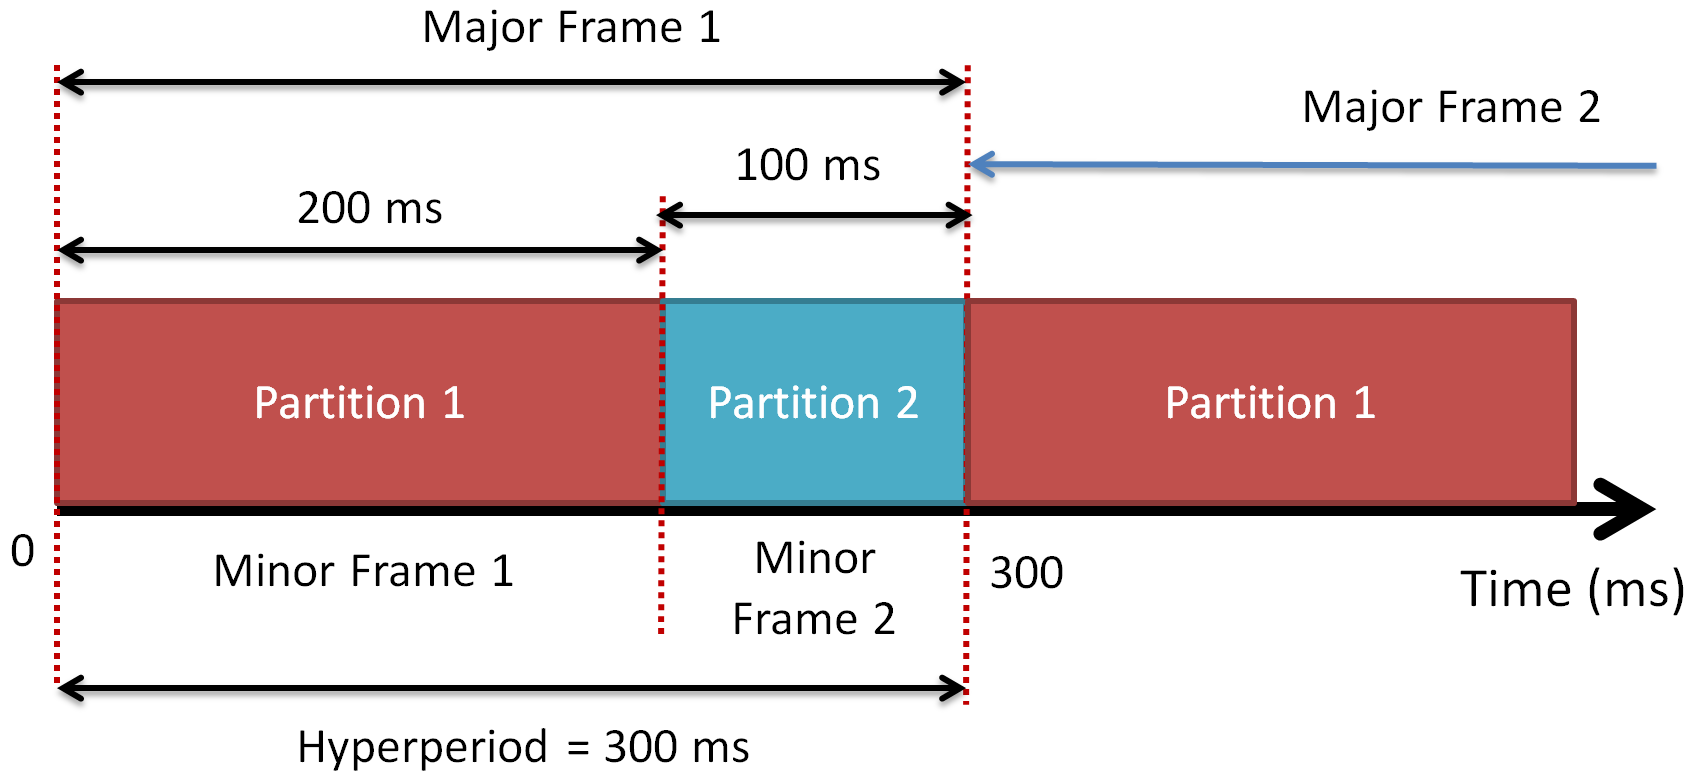
\includegraphics[width=\textwidth]{./figs/partition_scheduling}
	\caption{Sample Temporal Partition Schedule with Hyperperiod = 300 ms}
	\label{fig:partition_scheduling}
\end{figure}


Temporal partitions are periodic fixed intervals of the CPU's time. Threads associated with a partition are scheduled only when the partition is active. This enforces a temporal isolation between threads assigned to different partitions. The repeating partition windows are called \emph{minor frames}. The aggregate of repeating minor frames is called a \emph{major frame}. The duration of a major frame is called the \emph{hyperperiod}, which is typically the lowest common multiple of the partition periods. Each minor frame is characterized by a period and a duration. The period specifies how often this partition becomes active and the duration defines how much of the CPU time is available for scheduling the runnable threads associated with that partition. Figure \ref{fig:partition_scheduling} shows a sample temporal partition schedule. Each computing node in a network runs an OS scheduler, and the temporal partitions of the nodes are assumed to be synchronized, i.e. all hyperperiods start at the same time. Although the proposed analysis work tackles the challenges of a hierarchical scheduling scheme such as in DREMS, the presented analysis also studies cases without temporal partitioning, relying on the default Linux scheduling scheme.

The DREMS component model supports non-functional properties e.g. timeliness, fault tolerance and security as an integral part of the design. Every operation on a component is associated with a deadline that the developer specifies. Timed triggers can be associated with operations/callbacks that dictate when and how frequently certain operations are scheduled. Deadline monitoring is invoked when an operation is allowed to execute i.e. enqueued on the component message queue. The component thread that releases the business logic execution thread monitors the deadline. If a hard deadline is reached but the operation is incomplete, then the infrastructure notifies a local fault manager and appropriate actions are taken. 

Also, some long-term mission profiles e.g. space missions may involve long running computations and sensor-driven periodic calculations. Since the component execution semantics allows only one active operation to execute at a time within a component, it is possible that a ready operation is blocked for prolonged periods of time by an operation waiting on some I/O device. In such scenarios, developers can opt into using blocking I/O operations, polling mechanisms and asynchronous nonblocking I/O operations. In a blocking I/O task, the component is unavailable while the operation is running. Other components may execute in the system, but the one waiting on an I/O device is blocked. This blocking could propagate to other components and introduce significant delays. When using polling, some periodic task is scheduled that checks for the completion of I/O interaction. This leads to a potential waste of resources and decreased performance. Lastly, the component model supports asynchronous I/O, where the component triggers an I/O interaction and returns to handle other operations in the queue. The component does not block on the I/O and is notified when the I/O task completes. Such varied interaction patterns makes this component model very generic and a suitable target for our timing analysis work. The rich interactions and communication mechanisms are inspired by other common industrial component models such as CIAO \cite{CIAO_Chap:04} and ACM \cite{ACM_SPE:10}, and the execution semantics are precisely defined and implemented. A qualitative evaluation of its capabilities \cite{ISIS_F6_ISORC:13} show that although the model was designed for fractionated spacecraft, DREMS is suitable for a variety of distributed and embedded environments. 

\newpage
\subsection{Problem Statement}

Consider a set of mixed-criticality component-based applications that are distributed and deployed across a cluster of embedded computing nodes. Each component has a set of interfaces that it exposes to other components and to the underlying framework. Once deployed, each component functions by executing operations observed on its component message queue. Each component is associated with a single executor thread that handles these operation requests. The nature of mixed-criticality means that these executor threads are scheduled in conjunction with a known set of highly critical system threads and other low priority \emph{best-effort} threads. Furthermore, the application threads are also subject to a temporally partitioned scheduling scheme. System assumptions include:

\begin{enumerate}
	\item Knowledge about the component definition, component assembly, communication ports, deployment mapping, temporal partitioning etc. 
	
	\item Knowledge about the sequence of computation \emph{steps} of finite duration that are executed inside each component operation. This is dependent on the operation business-logic code written by the application developer.
	
	\item Knowledge of worst-case estimated time taken by the computational steps. There are some exceptions to this assumption e.g. blocking times on RMI calls cannot be accurately judged as these times are dependent on too many external factors.
\end{enumerate}

Using this knowledge about the system, the problem here is to ensure that the temporal behavior of the composed system meets its end-to-end timing requirements e.g. trigger-to-response times between distant sensors and actuators. Providing this guarantee implicitly requires that communicating components in a component assembly meet individual timing deadlines. Following the DREMS component model execution, a blocking I/O operation blocks a component from attending to any other requests till the operation is completed. Such blocking interaction patterns can propagate large delays to other components, especially in a highly connected system. A useful analysis result here would not only be in identifying end-to-end timing violations but also tracing delays within individual components. Tracking timing violations enables the analysis in identifying the causes for the anomalies e.g. nontrivial circular dependencies or scheduling delays. If an abstract model of the business logic of component operations is also encoded in the analysis model, then inefficient coding practices such as wasteful loops can also be marked as probable causes for deadline violations. 

Individual components need to be analyzed to identify the \emph{pure} execution times of the various computational steps in the component operations. When a set of tested components are composed together, each component's execution is affected by various factors including scheduling delays, network communication delays, blocking delays and other interaction-specific variabilities. Any timing analysis model for component-based software should account for such factors. As described in Section \ref{sec:simulation}, there are two important challenges to modeling and analyzing DRE systems: scope and abstraction level. The scope of the analysis here should be the full system of composed components. The abstraction level of the analysis must include enough detail to account for the various timing delays mentioned above while also not capturing all aspects of low-level code. A highly detailed and dynamic low-level model is necessary for simulation but not ideal for model checking and verification-based analysis due to issues like state space explosions. Also, highly composable system designs provide recombinant components that can be selected and assembled in various combinations to satisfy user requirements. In such cases, the analysis model must be efficiently capable of tackling changes in component assembly. This is a challenge when building and non-trivially generating an analysis model from a system design. Thus, efficiency, scalability and extensibility are also modeling requirements for our timing analysis.

\subsection{Challenges}

\subsubsection{Modeling Component-based Applications}

The CPN model should capture the behavioral semantics of our component model
described in \cite{ISIS_F6_ISORC:13}, using knowledge of several factors that resolve the deployment of the component-based application. These factors include the following system properties: (1) configuration of temporal partition scheduling on each node of the distributed system, (2) location of each component being deployed (which temporal partition and which computing node) (3) properties of the component executor threads (thread priority), (4) properties of timers (period and offset),
and (5) component interactions and assembly (i.e. the 'wiring'). The timing and behavior of the component interactions is dependent on both the application developer's business logic code and the distributed \emph{deployment plan}. Poorly written application code could cause circular dependencies, deadlocks or ever-growing message queues that are not easy to identify from a high-level system design model. The goal of the CPN model is to establish a simulation medium and an analysis framework that can identify and alert designers about such design inconsistencies. 

\subsubsection{Analysis Challenges}

Our CPN-based analysis methodology is a type of formal verification technique. There are several challenges to analyzing large DRE systems using formal verification methods like this. For an executable system model, a bounded state space needs to be generated. Here, the state space represents a tree of possible behaviors that the system can exhibit when executing from a known initial state. The state space should comprise of every possible combination of execution traces taken by system state variables. Once the evolution of state variables is recorded, state space analysis becomes a graph searching problem where given a state space graph of finite size i.e. fixed number of nodes and edges, how efficiently can the graph be searched to identify breakpoints or interesting graph nodes that represent positive or negative system states. The graph nodes each contain information about the system state variables e.g. execution time, thread state etc. By querying each node in the state space, system properties such as deadlock-freedom, deadline violations and trigger to response times can be deduced. Challenges to this problem include (1) state space explosion when the number of variables in the system grows, (2) efficiency of the searching algorithm e.g. memory consumption, worst-case search time etc., and (3) size of the bounded state space i.e. is the generated state space a complete representation of the system execution. The bound on the state space determines the validity of the state space analysis; the generated state space should span a much longer time compared to the periodicity of the DRE system being analyzed. The size of the generated state space is dependent on the amount of concurrency in the behavior e.g. if all the executing threads have unique priorities, the thread execution order is a constant as the scheduling is priority-based. However, for large systems with groups of applications and increased concurrency, an equally large state space is required to observe the tree of possible thread executions and operational behaviors.

From an analysis perspective, there are some important considerations that need to be made when building this CPN model. Foremost among these, is the issue of scalability. Here, a scalable analysis model needs to be efficient in two ways: (1) How does the CPN model grow in size with changes/additions to the system design model? Constructing/Generating a new CPN \emph{place} for each new added component port or hardware computer is not efficient because the CPN model would not scale well for large systems with hundreds of components; (2) How does the state space generated by the CPN model scale? How is the time taken to traverse the system state space affected when the analysis model has to handle hundreds of threads instead of tens of threads? These challenges need to be addressed for the analysis model to be useful in real-world DRE system scenarios e.g. airplane control systems and vehicle ECU networks.

\subsubsection{Generating CPN Analysis Model from System Design Model}

For large distributed applications, with multiple timers and component interaction patterns, hand-writing the CPN token specifications will prove to be both cumbersome and error prone. To avoid this, the temporal behavior specification discussed in Section \ref{sec:BL_Model} for component operations needs to be integrated into the system design model. Any part of a component e.g. timers, server ports, subscriber ports etc. that exposes an operation to the external environment needs to be \emph{tagged} with an abstract business logic model. This model describes the sequence of steps executed each time the operation is scheduled. Such models contain vital information that drives the CPN analysis execution. The business logic models, along with temporal partitioning specifications, component definitions and assembly, and the deployment plan need to be parsed, interpreted and translated. The system specifications derived from these sub-models need to be converted into Colored Petri net tokens that are injected into various parts of our generic CPN model. 

\subsection{The Choice of Colored Petri Nets}

With Colored Petri Nets (CPN) \cite{CPN}, tokens contain values of specific data types called colors. Transitions in CPN are enabled for firing only when valid colored tokens are present in all of the typed input places, and valid arc bindings are realized to produce the necessary colored tokens on output places. The firing of transitions in CPN can check for and modify the data values of these colored tokens. Furthermore, large and complex models can be constructed by composing smaller sub-models as CPN allows for hierarchical description.

One of the primary reasons for choosing Colored Petri Nets over other high-level Petri Nets such as Timed Petri Nets or other modeling paradigms like Timed Automata is because of the powerful modeling concepts made available by token colors. Each \emph{colored token} can be a heterogeneous data structure such as a \emph{record} that can contain an arbitrary number of fields. This enables modeling within a single \emph{color-set} (C-style \texttt{struct}) system properties such as temporal partitioning, component interaction patterns, and even distributed deployment. The token colors can be inspected, modified, and manipulated by the occurring transitions and the arc bindings. Component properties such as thread priority, port connections and real-time requirements can be easily encoded into a single colored token, making the model considerably concise. 

\subsection{Outline of Solution}

The top-level CPN Model is shown in Figure \ref{fig:hlcpn}. The places (shown as ovals) in this model maintain colored (typed) tokens that represent the states of interest for analysis e.g. the \emph{Clocks} place holds tokens of type \emph{clock\_token} maintaining information regarding the state of the clock values and temporal partition schedule on all computing nodes. 

\begin{figure}[h]
	\centering
	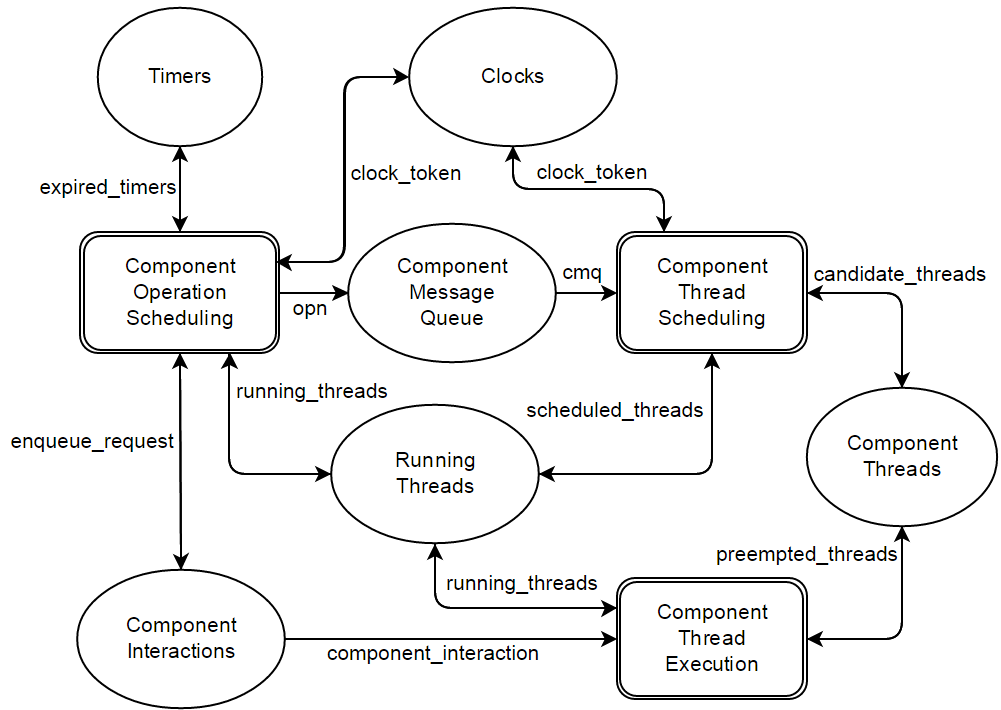
\includegraphics[width=0.9\textwidth]{./figs/HL_CPN}
	\caption{Hierarchical Colored Petri Net Analysis Model}
	\label{fig:hlcpn}
\end{figure}

The above model contains three hierarchical transitions that abstract low-level modeling details. These transitions handle component operation scheduling, OS thread scheduling, and execution, each progressing the hardware clocks appropriately. Transitions in Colored Petri nets can have \emph{priorities} i.e. a high-priority transition may be preferred over other enabled transitions in the marking. Although the low-level details of this model are not within the scope of this report, we believe that this model is effective in representing the complexities of component-based distributed real-time applications. Using a state space analysis engine, we analyze the state space of the parameterized model to compute useful system properties e.g. processor utilization, execution time plots etc. 

\subsection{Evaluation of Solution}
Rigorous evaluation of our solution is an important requirement for both justifying our approach and identifying its advantages and disadvantages. Evaluating our CPN-based analysis model requires us to probe both it's functional and behavioral aspects. The CPN model must accurately represent both the structural aspects of a software deployment e.g. process-to-hardware mapping, component operational steps etc. and the behavioral aspects e.g. thread scheduling, blocking effects, execution delays etc. This will be done by formally representing our DREMS component execution semantics and comparing this representation with our CPN formal model. Execution traces generated by CPN simulations for a variety of example cases would show the system elements modeled appropriately e.g. component operation scheduling, time-triggered periodic execution etc. Simulating both single-hardware and multi-hardware deployments presents us with trace data that can be compared with real-world deployments. Such comparisons, if equivalent, provide us the confidence required when selecting such an analysis model as an appropriate one. Similarly, the state space analysis will be evaluated by (1) forcing negative results e.g. deadlocks, deadline violations in the real system, then (2) modeling this system using our CPN analysis model, and (3) ensuring that the state space analysis process catches the timing violations. Since the presence of a timing violation in the CPN analysis does not necessitate a timing anomaly in the real-system, the opposite scenario is forced for the purpose of evaluation. Lastly, with peer-review evaluation of the structural and behavioral CPN model of the DREMS system, the design-model to CPN model translation is implicitly evaluated too. By forcing the frequent use of the \emph{CPN Analysis Model Generator}, we evaluate the translation rules for a wide range of examples. 

\subsection{Contributions}

\subsubsection{Colored Petri Net-based Model}
We designed and built a Colored Petri net-based extensible and scalable analysis model of distributed component-based applications. Several CP-nets are used to compose the different layers of the design model e.g. hierarchical scheduling, network-level interactions etc. This modeling paradigm was reported \cite{kumar2014colored} with a simple \emph{Trajetory Planner} example - a distributed real-time scenario with temporal partitioning and a combination of interaction patterns supported by DREMS, including synchronous remote procedure calls and anonymous publish/subscribe message passing schemes. Improvements to this model have since been made and are discussed in later sections. 

\subsubsection{State Space Analysis and Verification of Safety-critical System Properties}
We used the prototype CPN analysis model and performed bounded state space analysis using both the in-built state space analysis tool in CPN Tools \cite{CPNTools} and also user-defined application-specific queries e.g. deadline violation checks, partial thread execution order generation etc. Here, tokens in CPN places, in each marking, encode the state of the system at that marking (time instant). State space analysis yielded positive results \cite{kumar2014colored} identifying deadline violations, deadlocks, worst-case trigger-to-response times, and partial thread execution orders in a variety of scenarios. Scalability testing proved the CPN model to be effective for medium-large sized component-based applications - tested with up to 100 components distributed on up to 10 computing nodes. 


\subsubsection{Design Model to Analysis Model Translation}
A \emph{CPN Generator} model interpretor \cite{kumar2014colored} was developed to generated Colored Petri net analysis models from system designs. This interpreter parses the design model tree, identifies system properties such as component definitions, port properties, scheduling schemes etc. and constructs an interpreted data structure (tree). Using this tree, system properties are converted to relevant CPN token strings. Using T4 Text Templates \cite{T4TextTemplates} in a Visual Studio environment, the generated strings were embedded into a generic CPN text template by a templating engine. The end result is a parameterized Colored Petri net (.cpn) file that can analyze the system. Since then, we have also ported this generator to a Python-based development environment \cite{kumarROSMOD} and performed further testing.

\newpage
\section{Modeling Component Operation Business Logic}
\label{sec:BL_Model}

\subsection{Problem Statement}

Consider a set of component-based applications deployed on distributed hardware. Each applications consists of groups of components that interact with each other and also with the external environment e.g. I/O devices, other applications, underlying middleware etc. Each component exposes a set of interfaces through which external entities can request \emph{operations}. As mentioned earlier, an operation is an abstraction for the different tasks undertaken by a component. These operations are exposed through ports and can be requested by other components. When an operation is requested, the request is placed in the component's message queue and eventually serviced. When ready, the business logic of the operation i.e. a local callback is executed. This piece of code represents the brains of the operation. Our goal here is to be able to model this business logic, for every component operation, effectively as part of the design model, including temporal estimates such as worst-case execution times for individual code blocks, so that the model can be translated into appropriate data structures in our CPN analysis model.

\subsection{Challenges}

The execution of component operations service the various periodic or aperiodic interaction requests coming from either a timer or other connected (possibly distributed) components. Each operation is written by an application developer as a sequence of execution steps. Each step could execute a unique set of activities, e.g. perform a local calculation or a library call, initiate an interaction with another component, process a response from external entities, and it can have data-dependent, possibly looping control flow, etc. The behavior derived by the combination of these steps contribute to the worst-case execution of the component operation. The behavior may include non-deterministic delays due to component interactions while being constrained by the temporally partitioned scheduling scheme and hardware resources. The challenge here is to identify a metamodel grammar that would represent the potentially dynamic behavior realized in a component operation. The modeling aspects emerging from this challenge will have to propagate to any timing analysis model that studies the system. This is true because any non-deterministic delays such as blocking times need to be accounted for when analyzing the temporal behavior.

\subsection{Outline of Solution}
The business-logic model of a component operation requires to be completely integrated into our CPN modeling methodology. This means that the model, however complex, needs to be translated into some token data structure in CPN. This is our primary constraint. The CPN analysis model needs to know how an operation is structured i.e. what are the sequential steps in the code, along with WCET on each step. Lastly, since the CPN model does not model or simulate component data management, data-dependent conditional statements in the business-logic model were avoided or abstracted away. Following these rules, we designed a metamodel for the component operation business logic. Each component operation model is then attached to a component port or timer in the main design model and enriches the model with refined details about the workings of the operation. In summary, this model is capable of representing several types of code blocks including local function calls, remote procedure calls, outgoing port-to-port interactions, incoming port-response processing, and bounded loops.

\subsection{Evaluation of Solution}
Evaluating the business logic grammar is important for two reasons. If the business logic modeling grammar is not sufficiently rich, then the model would not accurately represent the actual implementation code and this breaks any results obtained by CPN analysis. Secondly, preprocessing the business logic models helps system integrators analyze component interactions for unsafe interaction patterns e.g. cyclic dependencies, potential deadlocking behaviors etc. This implicitly constrains application developers about the types of operational steps that are permitted when programming real-time component-based systems. Evaluating the accuracy of the business-logic model will be done over a wide range of samples, compared against the implementation code to check for abstract correlation. The drawbacks and limitations of this grammar will be identified and potential improvements will be implemented. The final step in the evaluating the correctness of such models involves in checking the expected execution times of each operational step, as expressed in the models. This is done by executing the component operation on the real-system while ensuring the absence of other interfering threads, and identifying the WCET of individual code blocks using monitoring methods e.g. logging. This experimental evaluation is described later in Section \ref{sec:Experimental_Evaluation}.

\subsection{Contributions}
We have presented an approach \cite{SEUS} for modeling the operational behavior of each component in an application. The modeling grammar uses a sequence of timed steps that are executed by the operation, including interaction patterns. This approach enables abstracting the details of the middleware, while representing the temporal behavior of the component business logic.

\newpage

\section{Modeling and Analysis Improvements}
\label{sec:Improvements}

\subsection{Problem Statement}

The CPN analysis work presented in \cite{kumar2014colored} has some limitations. The clock values in the distributed set of computing nodes progress by a fixed amount of time regardless of the pace of execution. This is one of the primary causes of state space explosion since many of the intermediate states between \emph{interesting} events, though uneventful, are still recorded by the state space generation. For instance, in a temporal partition spanning 100 ms, even if a thread executes for 5 ms and the rest of the partition is empty, then if the clock progresses at a 1 ms rate, a 100 states are recorded in the state space when there are atmost 5-7 interesting events in this interval. For a larger set of distributed interacting components, this can become a problem. Also, for distributed scenarios where multiple instance of a set of applications are executed in parallel, in independent computers, our CPN modeling methodology isn't efficient, leading to a tree of parallel executions even when the distributed computers are independent i.e. the computers can be synchronously progressed. The goal of this work is to mitigate such analysis issues and arrive at a more efficient and scalable analysis model. 

\subsection{Outline of Solution}
Improving the performance of our CPN analysis method required the evaluation of our existing results to identify how the state space generation worked. The state space of CPN is a tree of CPN \emph{markings}, where each marking is a data structure representing the tokens in all it's places. So, our goal is to reduce the number of markings accumulated in the CPN i.e. the number of distinct states of interest. This required us to evaluate our representation of time. Using time as a fixed-step monotonically increasing entity means that the CPN place managing time would always contain a new \emph{clock token}, therefore forcing the CPN marking to become a part of the state space.
To alleviate this issue, we modeled time as a dynamically changing variable, where the changes are strategically forced \emph{time jumps} instead of a statically increasing clock value. Similarly, our data structure representation for distributed deployments i.e. using unordered token sets instead of ordered lists, enabled our earlier CPN models to nondeterministically choose one of the various distributed nodes to execute, generating a exponentially increasing tree of execution orders. Once we moved to representing our distributed hardware nodes as a list, the execution engine iteratively executing the analysis on each node in the list, leading to one execution order instead of a tree. 

\subsection{Evaluation of Solution}
Drastic changes to our CPN analysis e.g. representation of time, becomes risky when such changes are accompanied by unexpected execution behaviors. Enforcing time jumps requires strict semantic rules that need to be carefully judged e.g. jumping in time to the next timer expiry $t_{e}$ on Hardware $BBB\_1$ should not happen until all foreseen executions, interactions and triggers on all other nodes $BBB_2 ... BBB_n$ within the time frame $t_{now}$ to $t_e$ are executed. Following such rules on each hardware node, and on each calculated time jump leads to a safer execution. This is required because erroneous time jumps can lead to a crippled CPN model with inconsistent execution traces. Evaluating analysis improvements like time jumps requires large sets of unit tests with various types of examples, enforcing every time jump rule. Identifying erratic execution patterns leads to an improved set of rules and a more robust analysis model. Thus, this solution will be evaluated with a wide range of examples, enforcing various combinations of time jumps and component interactions to identify flaws, using state space analysis, in the heuristics. 

\subsection{Contributions}

Such issues are resolved with our analysis improvements, reported in \cite{SEUS}. We modified the timing analysis model to allow dynamic time progression i.e. the clocks (one for each computing node) in the CPN model do not progress at a constant rate but instead experience \emph{time jumps} to the next interesting time step e.g. next timer expiry, end of partition or next scheduling preempt point. This makes the system execution progress at a much higher rate and reduces the overall number of states being recorded in the state space. We also adjusted our modeling concepts when describing distributed deployments. We experienced needless state space explosions as a consequence of using CPN semantics when modeling distributed computers. If the computers are modeled as an aggregate of independent CPN tokens, then the CPN transition that progresses the execution in each computer is independent, leading to a potential $C!$ different orders for $C$ computers. For instance, 4 distributed computers leads to 24 possible execution orders displayed by the transition responsible for \emph{picking} the next computer to evaluate and progress. We alleviate this issue by assuming that all computers in a distributed scenarios have synchronized clocks and execute simultaneously leading to a synchronous progress. This is done by maintaining the state of each computer in a \emph{list} instead of an unordered aggregate. This approach is inspired by the symmetry method for state space reduction \cite{Kristensen2000}. These improvements are evaluated in \cite{SEUS}, where we detail our solutions with motivating examples. 


\if 0
\subsection{Handling Time}
\label{handling_time}

The CPN-based analysis consists of executing a simulation of the model and constructing a state space data structure for the system (for a finite horizon), and then performing queries on this data structure. This is automated by CPN Tools. The first improvement over the basic CPN approach is in how we handle time. Although it is true that CPN and similar extensions to Petri Nets such as Timed Petri Nets inherently have modeling concepts for simulation time, we explicitly model time as an integer-valued \emph{clock} color token in CPN. There are several reasons for this choice. 

Firstly, this is an extension to our previous arguments about choosing Colored Petri Nets. Modeling the OS scheduler clock as a colored token allows for extensions to its data structure such as (1) intermediate time stamps and internal state variables, and (2) adding temporal partitioning schemes like the (time-partitioned) ARINC-653 \cite{ARINC-653} scheduling model (Figure \ref{fig:clock}). 

\begin{figure}[h]
	\centering
	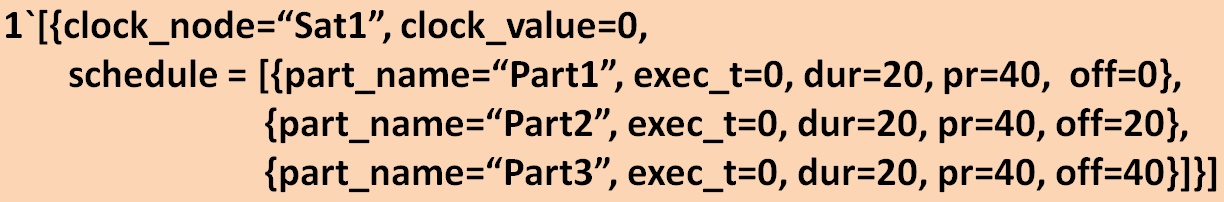
\includegraphics[width=0.7\textwidth]{./figs/clock}
	\caption{A Clock Token with Temporal Partitioning}
	\label{fig:clock}
\end{figure}

These extended data structure fields can be more easily manipulated and used by the model transitions during state changes, allowing for richer modeling concepts that would not be easily attainable using token representations provided by Timed Petri Nets. The ability to pack colored tokens with rich data structures also reduces the total number of colors required by the complete model. This quantitative measure directly influences the reduced size of the resultant state space. The downside of this approach to modeling is that we have to choose a time quantum. But in practical systems this is usually not a problem, as the low-level scheduling decisions are taken by an OS scheduler based on a time scale with a finite resolution. We have chosen 1 msec as the quantum (corresponding to the typical 1KHz scheduler in Linux), but it can be easily changed. 

Secondly, modeling time as a token allows for smarter time progression schemes that can be applied to control the pace of simulation. If we did not have such control over time, the number of states recorded for this color token would eventually explode and itself contribute to a large state space. In order to manage this complexity, we have devised some appropriate \emph{time jumps} in specific simulation scenarios. 

If the rate at which time progresses does not change, then for a 1 msec time resolution, \emph{S} seconds of activity will generate a state space of size: $SS_{size} = \sum\limits_{i=1}^{S*1000} TF_{t_i}$ where $TF_{t_i}$ is the number of state-changing CPN transition firings between $t_i$ and $t_{i+1}$. This large state space includes intervals of time where there is no thread activity to analyze either due to lack of operation requests, lack of ready threads for scheduling, or due to temporal partitioning. During such idle periods, it is prudent to allow the analysis engine to \emph{fast-forward} time either to (1) the next node-specific clock tick, (2) the next global timer expiry event, or (3) the next activation of the node-specific temporal partition (whichever is earliest and most relevant). This ensures that the generated state space tree is devoid of nodes where there is no thread activity.

\begin{figure}[h]
	\centering
	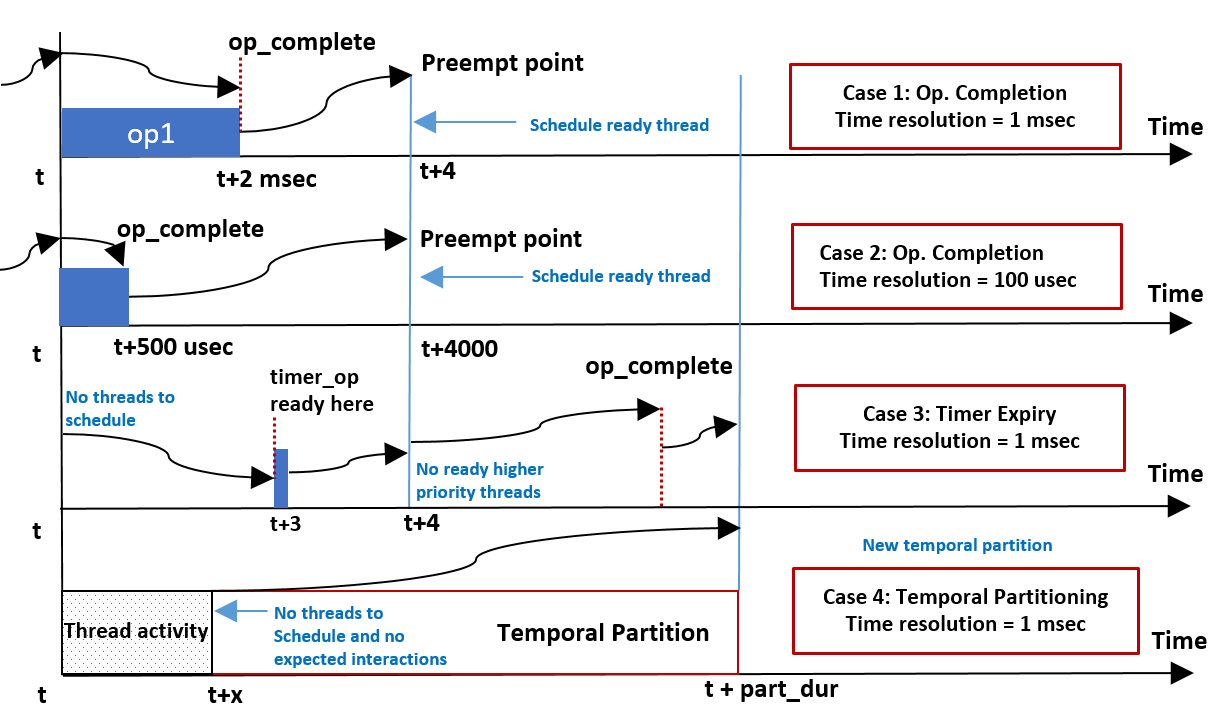
\includegraphics[width=\textwidth]{./figs/time}
	\caption{Dynamic Time Progression}
	\label{fig:time}
\end{figure}

Figure \ref{fig:time} illustrates these time jumps using 4 scenarios. Assuming the scheduler clock ticks every 4 msec, Case 1 shows how time progression is handled when an operation completes 2 msec into its thread execution. At time t, the model identifies the duration of time left for an operation to complete. If this duration is earlier than the next preempt point, then there is no need to progress time in 1 msec increments as no thread can preempt this currently running thread till time t + 4 msec. Therefore, the \emph{clock\_value} in Figure \ref{fig:clock} progresses to time t + 2 msec, where the model handles the implications of the completed operation. This includes possibly new interactions and operation requests triggered in other components. Then, time is forced to progress to the next preempt point where a new candidate thread is scheduled. This same scenario is illustrated in Case 2 when the time resolution is increased to 100 usec instead of 1 msec. Notice that the number of steps taken to reach the preempt point are the same, showing how the state space doesn't have to explode simply because the time resolution is increased. Case 3 illustrates the scenario where at time t, the scheduler has no ready threads to schedule since there are no pending operation requests but at time t + 3 msec, a component timer expires, triggering an operation into execution. Since timers are maintained in a global list, each time the \emph{Progress\_Time} transition checks its firing conditions, it checks all possible timers that can expiry before the next preempt point. So, at time t when no threads are scheduled, the model immediately jumps to time t + 3. This scenario also shows that if the triggered operation does not complete before the preempt point \emph{and} there are no other ready threads or timer expiries that can be scheduled, the clock value jumps to the operation completion. It must be noted here that this case is valid only because the DREMS architecture we have considered uses a non-preemptive operation scheduling scheme. Lastly, Case 4 shows time jumps working with temporal partitioning. At some time t + x, the model realizes the absence of ready threads and does not foresee any interaction requests from other components, then it safely jumps to the end of the partition without stepping forward in 1 msec increments. This time progression directly shows how the state space of the system execution reduces while still preserving the expected execution order, justifying our choice of modeling time as a colored token using CPN. 

\subsection{Distributed Deployment} 
\label{distributed_deployment}

The second structural change to the analysis model is in how distributed deployments are modeled and simulated. Early designs on modeling and analysis of distributed application deployments \cite{kumar2014colored} included a unique token per CPN place for each hardware node in the scenario. Since the individual \emph{node} tokens are independent and unordered, there is nondeterminism in the transition bindings when choosing a hardware node to schedule threads in. For instance, if there are 2 hardware nodes in the deployment with ready threads on both nodes, then either node can be chosen first for scheduling threads leading to two possible variations of the model execution trace. Therefore the generated state space would exponentially grow for each new hardware node. In order to reduce this state space and improve the search efficiency, we have merged hardware node tokens into a single \emph{list} of tokens instead of a unassociated grouping of individual node tokens. This approach is inspired by the symmetry method for state space reduction \cite{Kristensen2000}.

\begin{figure}[h]
	\centering
	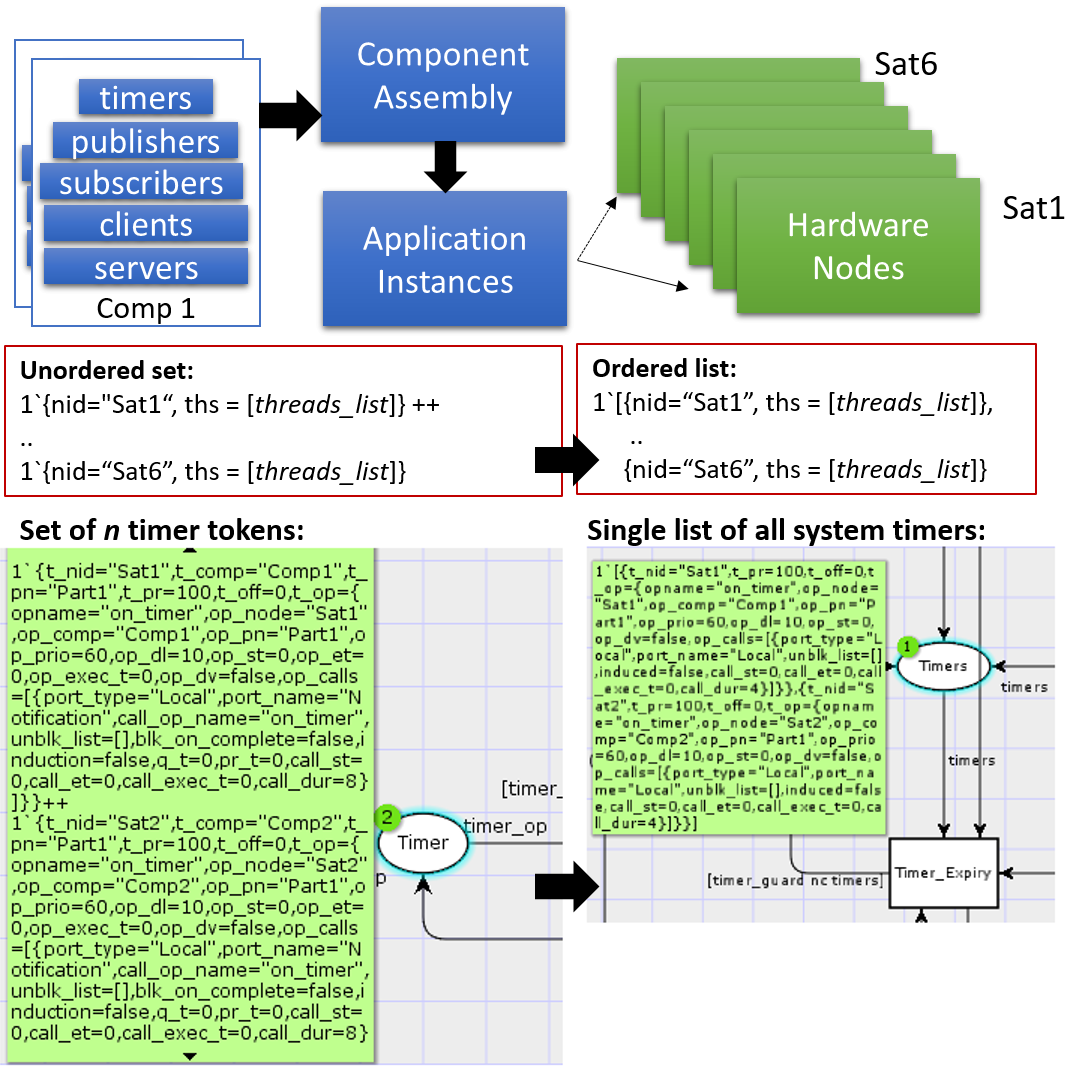
\includegraphics[width=0.8\textwidth]{./figs/dd}
	\caption{Structural Reductions in CPN}
	\label{fig:dd}
\end{figure}



Figure \ref{fig:dd} illustrates this structural reduction. Consider a distributed deployment scenario with an instance of a DREMS application deployed on each hardware node, Sat1 through Sat6. Components \emph{Comp1} and \emph{Comp2} are triggered by timers, eventually leading to the execution of component operations (modeled as shown in Figure \ref{fig:ebnf}). If all the timer tokens in the system were modeled individually, the transition \emph{Timer\_Expiry} would non-deterministically choose one of the two timer tokens that are ready to expire at \emph{t=0}. However, if the timers are maintained as a single list, then this transition (1) consumes the entire list, (2) identifies all timers that are ready to expire, (3) evaluates the timer expiration function on all ready timers, (4) propagates the output \emph{operation} tokens to the relevant component message queues in a single firing. This greatly reduces the tree of possible transition firings and therefore the resultant state space. Also, if there is no non-determinism in the entire system, i.e., there is a distinct ordering of thread execution, then this model can be scaled up with instantiating the application on new hardware nodes with no increase in state space size. This is because all of the relevant tokens on all nodes are maintained as a single list that is completely handled by a single transition firing. 

An important implication of the above structural reduction is that the simulation of the entire system now progresses in synchronous steps. This means that at time 0, all the timers in all hardware nodes that are ready to expire will expire in a single step. Following this, all operations in all component message queues of all these nodes are evaluated together and appropriate component executor threads are scheduled together. When these threads execute, time progresses as described in Section \ref{handling_time}, moving forward by the minimum amount of time that can be fast-forwarded.
\fi

\newpage
\section{Investigating Advanced State Space Analysis Methods}

\subsection{Problem Statement}
State space analysis techniques have been successfully applied with Colored Petri Nets in a variety of practical scenarios and industrial use cases \cite{CPN_0}, \cite{CPN_1}. The basic idea here is to compute all reachable states of the modeled concurrent system and derive a directed graph called the state space. The graph represents the tree of possible executions that the system can take from an initial state. It is possible from this directed graph to verify behavioral properties such as queue overflows, deadline violations, system-wide deadlocks and even derive counterexamples when arriving at undesired states. 

Advanced state space analysis techniques arise from the need for efficient space space searching algorithms. State space analysis is challenged by time, memory, and computational power. Large state spaces require large CPU RAM and efficient search methodologies to quickly arrive at a useful result. With increasingly complexity in system designs, the number of state variables to store in memory also increases. Our problem here is to identify and apply advanced state space analysis techniques, applicable in the context of our CPN model and available as tested analysis tools that mitigate such complexities in state space analysis. This will help improve the scalability of our model and also reduce the memory footprint of the analysis. 

\subsection{Outline of Solution}

The variety of CPN-specific state space reduction techniques \cite{CPN_Sweepline}, \cite{CPN_Symmetry} developed in recent times has significantly broadened the class of systems that can be verified. In order to easily apply such techniques to our analysis model, we use the ASAP \cite{ASAP} analysis tool. The tool provides for several search algorithms and state space reduction techniques such as the \emph{sweep-line method} \cite{Christensen2001} which deletes already visited state space nodes from memory, forcing on-the-fly verification of temporal properties. The main advantage of such techniques is the amount of memory required by the analysis to verify useful properties for large models. 

The sweep line method for state space reduction is used to check for important safety properties such as lack of deadlocks, timing violations etc. using user-defined model-specific queries. Practical results enumerated in \cite{Christensen2001} show improvements in time and memory requirements for generating and verifying bounded state spaces. The method relies of discarding generated states on-the-fly by performing verification checks during state space generation time. Any state that does not violate system properties can be safely deleted. Another advantage of this method compared to similar reduction methods such as bit-state hashing \cite{CPN_Bitstate_Hashing} is that a complete state space search is guaranteed. 

\subsection{Evaluation of Solution}
We will evaluate these advanced state space analysis methods by comparing the obtained results with our basic state space analysis in CPN Tools. Using several criteria such as state space generation time, state space query generation, query processing time, memory usage etc., we can generate a comparison table to show the overall improvements in the analysis workflow. Advanced analysis techniques are usually accompanied by some expertise requirements that can be masked by nicely designed analysis tools. Our goal with ASAP is to use a model-driven approach to enable advanced analysis methods that does not require much expertise. With ASAP, we are able to generate verification project templates i.e. building blocks much like Simulink that are wired up together and provide an interface to the low-level analysis engine. Therefore, evaluation of this work requires both the evaluation of the advanced methods applied, and the tool used. As for the analysis methods applied, it is important to ensure that the state space tree, with all of the applied analysis heuristics, is still sufficiently probed when searching for system properties. Heuristics that enable state space analysis but only by partially checking the tree can lead the case where the state space analysis does not identify timing errors because of the incomplete search. This will be checked with negative test cases where the design model is known to be flawed; if the results from ASAP identify injected timing errors for all test cases, then the analysis is sound. 

\subsection{Contributions}
These methods were evaluated on our CPN analysis method and the results were presented in \cite{SEUS}. We used a large and diverse 100 component-based application for our testing. Using the CPN Tools' built-in state space analysis tool, a bounded state space of thread activity was generated. The state space generation took 36 minutes on a typical x86 laptop. We imported the same CPN analysis model onto ASAP and performed on-the-fly verification checks for lack of dead states in the analysis model for the same bounded state space. The on-the-fly verification, without any graphical interface overheads, took less than 10 minutes to compute a lack of system-wide deadlocks. It must be noted here that this improved result is due to not only because of the efficient state space search but also because of symmetry-based structural reduction discussed in the previous section.

\if 0

In order to illustrate the utility of such state space reduction techniques, we consider a large-scale deployment. Figure \ref{fig:gm} shows the generated CPN model for a domain-specific DREMS application. This is a scaled-up variant of several satellite cluster examples we have used in previous publications \cite{DREMS13Software, kumar2014colored}. The example consists of a group of communicating satellites hosting DREMS applications. The component assembly for this application consists of 100 interacting components distributed across 10 computing nodes, many of which are triggered by infrastructural timers. Notice in Figure \ref{fig:gm} how there is only one token in each of the main CPN places, as described in Section \ref{distributed_deployment}. All of the component timers are appended to the list maintained in \emph{Timers} place. Similarly, all node-specific clock tokens are maintained in place \emph{Clocks}.  

\begin{figure}[h]
	\centering
	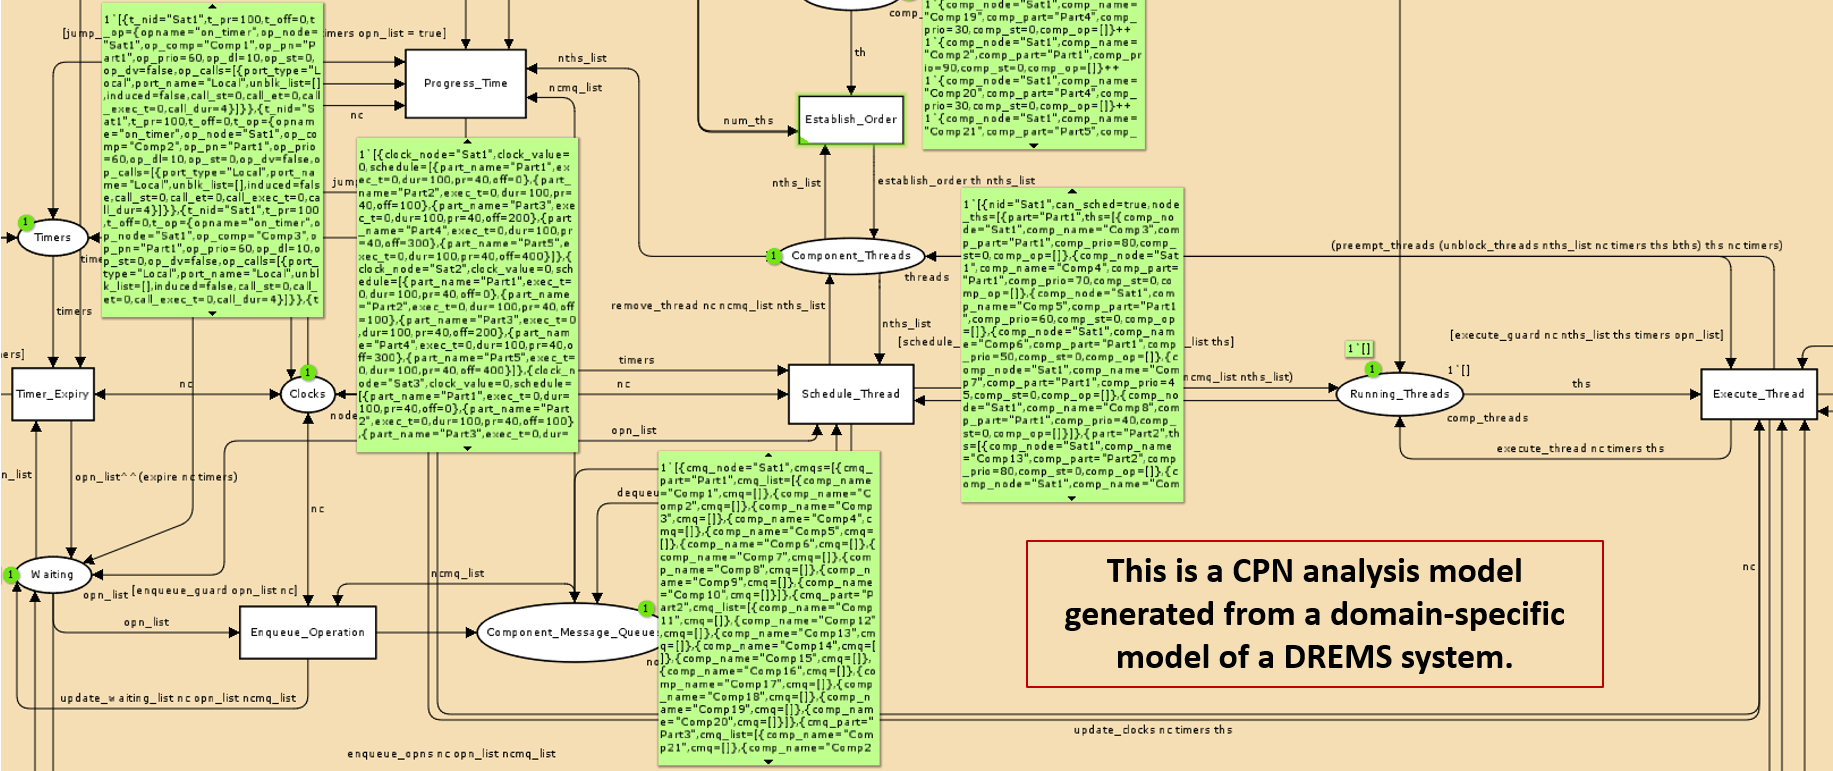
\includegraphics[width=\textwidth]{./figs/Generated_Model}
	\caption{Generated CPN model for a Distributed Application Deployment}
	\label{fig:gm}
\end{figure}

At time \emph{t=0}, before the simulation is kicked off, the transition \emph{Establish\_Order} generates the powerset of thread execution orders that are possible given the configuration of the clock token. This may be a potentially large set depending on the number of threads of equal priority in each partition. Once this tree of possible orders is established, the complete set of timers that are ready to expire are evaluated. Each timer expiry manifests as an operation request and each callback operation modeled using the grammar shown in Figure \ref{fig:BL_Model}. Once the operations are ready to execute, the highest priority component thread with a pending operation request is chosen for execution. This thread scheduling happens on all hardware nodes. When each thread executes, new interactions may occur as a consequence of the execution. For instance, if a component thread executes a timer operation in which the component publishes on a global topic, the consequence of this action would include a set of callback operation requests on all components that contain subscribers to that global topic. Lastly, all running threads are evaluated to identify the minimum amount of time that can be safely fast-forwarded in each node. If the running component threads are independent or symmetrical, then the maximum possible time progression is up to the end of the temporal partition. Note here that temporal partition in the deployment can be set to an empty list which simply removes the  partitioning constraint and treats all component threads on a node as candidate threads for execution. The above sequence of transitions repeat for as long as there is a timer expiry, a pending operation request or an unfinished component interaction. 

\begin{figure}[h]
	\centering
	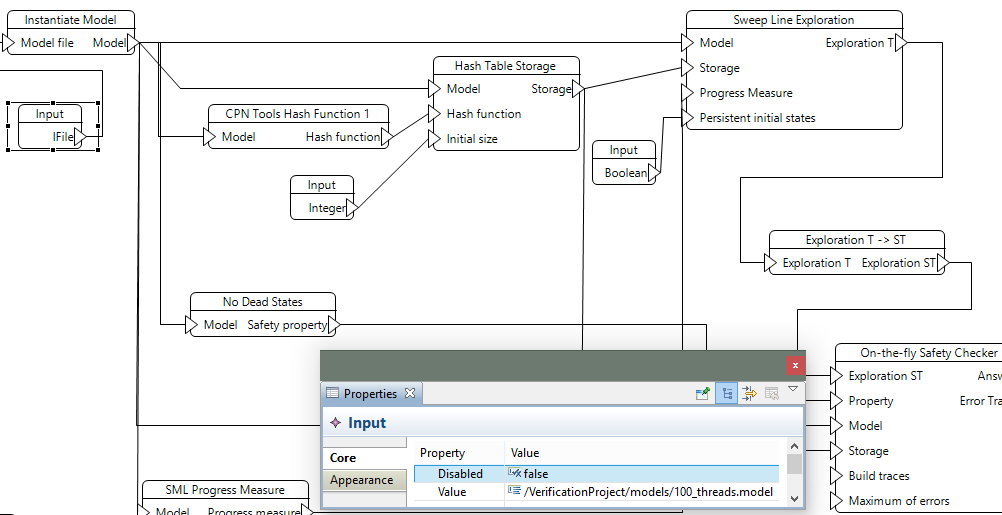
\includegraphics[width=\textwidth]{./figs/sl}
	\caption{Sweep-Line Method}
	\label{fig:sl}
\end{figure}

Using the CPN Tools' built-in state space analysis tool, a bounded state space was generated reaching up-to 20 hyperperiods of component thread activity. This bounded generation took 36 minutes on a typical laptop. Our goal with such an example is to evaluate the effectiveness and utility of state space reduction techniques with respect to speed and memory usage. Figure \ref{fig:sl} shows a simple block diagram of the sweep-line method as configured in ASAP. Performing on-the-fly verification checks for lack of dead states in the analysis model, results indicate lack of system-wide deadlocks due to blocking behaviors triggered by RMI-style synchronous peer-to-peer interaction patterns. Figure \ref{fig:ds} shows analysis results obtained from a \emph{Verification Job} executed in the tool. Notice the on-the-fly verification taking less than 10 minutes to perform deadlock checks on this sample deployment. Using the \emph{Palette} in ASAP, several standard ML (SML) user queries can be created to check for domain-specific properties. 

\begin{figure}[h]
	\centering
	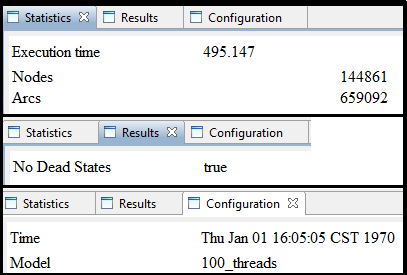
\includegraphics[width=0.6\textwidth]{./figs/asap}
	\caption{Dead States Checking in a Component-based application}
	\label{fig:ds}
\end{figure}

It must be noted here that this improved result is due to not only because of the efficient state space search but also because of symmetry-based structural reduction discussed in the previous section. If not for this reduction, the state space search requirements would exponentially grow for each new hardware node added to the deployment. 
\fi

\newpage
\section{Experimental Validation of Timing Analysis Results}
\label{sec:Experimental_Evaluation}

\subsection{Problem Statement}

Experimentally validating our timing analysis results is an important and necessary requirement. In order to obtain any level of confidence in our CPN-based work, the system design model needs to be completed implemented, and deployed on the target hardware platform. We have constructed a testbed \cite{kumarTestbed} to simulate and analyze resilient cyber-physical systems consisting of 32 Beaglebone Black development boards \cite{BBB}. We have chosen the light-weight ROS \cite{ROS} middleware layer and implemented our ROSMOD Component model \cite{kumarROSMOD} on top of it. This component model provides the same execution semantics and interaction patterns as our DREMS component model \cite{ISIS_F6_ISORC:13}. Our goal with this work is to (1) establish a set of distributed component-based applications, (2) translate this design model to our CPN analysis model, (3) deploy these applications on our testbed and accurately measure operation execution times, and finally (4) perform state space analysis on the generated CPN model to check for conservative results, compared against the real system execution.

\subsection{Challenges}

Experimental validation requires that online measurements of the real-time system match with the timing analysis results in a way that the timing analysis results are always close but conservative. If the timing analysis results predict a deadline violation, this does not necessarily mean that the real system will violate deadlines but if the timing analysis and verification guarantees a lack of deadline violations, then the real system should follow this prediction. One of the biggest assumptions in our CPN work is the knowledge of worst-case execution times of the individual steps in the component operations. There are various ways to obtain the WCET values for individual operational steps but the easiest approach is to execute the design into our testbed and make accurate measurements.

WCET of component operational steps needs to be measured by having the component operation execute at real-time priority with no other component threads intervening this process. This measurement gives us a \emph{pure execution time} of the code block. The process must be repeated for all component operations to obtain meaningful worst-case estimates that are tailored to the target platform. Obtaining the WCET values by this method is not only more realistic but also an accurate representation of the target system. Once these individual numbers are obtained, the values are plugged into the CPN through our business-logic models. Ideally, the CPN model, consisting of a composition of component operation models, when analyzed, produces results that closely resemble a real-system deployment of the component assembly. Such results would validate the modeling accuracy and the analysis results.

\subsection{Evaluation of Solution}
Experimentally validating our timing analysis results requires some careful evaluation. Such evaluation will include the testing parameters e.g. operating system, thread scheduler clock \emph{tick}, clock difference between nodes in distributed deployments etc. These factors play an important role in the execution traces observed for the tested applications. Since we are deriving WCET for operational steps from experiments, the experimental tests should be performed in \emph{sterile} environments i.e. no other interfering threads or interactions besides the tested application components. Secondly, the monitoring of such applications will be performed with minimum possible overhead e.g. cyclic buffers for logging. Thirdly, each test will be run multiple times to obtain an average set of resultant behaviors to compare our CPN results against. This is necessary because testing methodologies, especially using prototype hardware can never be exhaustive. In summary, we will (1) execute our component-based test applications on a  distributed set of Beaglebone Black development boards, (2) obtain middleware-level and application-level debug logs, (3) post-process these logs to generate execution time plots, and (4) compare these execution time plots to state space analysis results obtained using our CPN analysis model.

\subsection{Proposed Contributions}
We will use our resilient CPS testbed to run experimental deployments of a variety of component-based distributed real-time scenarios. By executing component threads individually and at real-time priority, an execution profile i.e. pure execution times of the individual code blocks in component operations is obtained. The above measurements are obtained using a low-overhead logging framework that hooks into the component middleware and uses C++'s chrono high-resolution timers to record time instances in nanoseconds. We have a Python log analysis script that parses the component instance logs, identifies the time stamps at which operations are enqueued, dequeued and completed to generate execution plots that illustrate the component behavior. We will translate these results into business logic models and generate CPN timing analysis models, one per deployment. We will perform state space analysis and verification on the generated CPN analysis models and obtained execution plots of specific traces. We will compare the CPN analysis plots with the plots obtained by post-processing real execution logs. This comparison should indicate that the analysis model is consistently describing and analyzing the scenarios and providing conservative but close results.

\newpage
\section{Modeling and Analysis of Long-Running Component Operations}

\subsection{Problem Statement}

Our DREMS component model implements a non-preemptive component operation scheduling scheme. A component operation that is in the queue, regardless of its priority, must wait for the currently executing operation to run to completion. This is a strict rule for operation scheduling and does not work best in all system designs e.g. in a long-running computation-intensive application, rejuvenating the executing operation periodically and restarting it at a previous checkpoint increases the likelihood of successfully completing the application execution. In applications executing long-running artificial intelligence (AI) search algorithms e.g. flight path planning algorithms, the computation should not hinder the prompt response requirements of highly critical operation requests such as sudden maneuver changes. Our DREMS component model does not support the \emph{cancellation} of long-running component operations to service other highly critical operations waiting in the queue. Our goal is to model and analyze component-based systems that support long-running operations, with checkpoints, that enable the novel integration of AI-type algorithms into our design and analysis framework. 

\subsection{Challenges}

We need to identify the semantics of a long-running component operation i.e. the scenarios under which the component operations scheduler cancels a long-running operation in favor of some other operation waiting in the queue. If a long-running computation is modeled as a sequence of execution steps with equally-spaced checkpoints, then the operation would execute one step at a time and the scheduler would wait for the nearest checkpoint to reach, before canceling the operation (if needed). An important challenge here is accurately identifying the priority difference between the long-running operation and the waiting operation. If the long-running operation is one checkpoint away from completion e.g. 100-200 ms of execution time, then strictly following our cancellation rules would not be the most prudent choice since this operation is almost complete. However, if the waiting operation is a critical one, then regardless of the state of the long-running operation, the executing operation must be canceled. Secondly, the modeled long-running computation semantics must be incorporated into our component model so that any analysis results obtained can be suitably validated. 

\subsection{Outline of Solution}
We are modeling long-running computations just like any other component operation, as outlined in Section \ref{sec:BL_Model}. However, in each long-running operation, we will include a synchronous \emph{checkpoint step}. The only assumption we make about this long-running operation is the periodicity of these checkpoint steps i.e. we know how frequently a new checkpoint is reached and we assume that the search algorithm used by the long-running operation is capable of reaching a safe state (the checkpoint) before canceling itself if required. If a higher priority operation is ready and waiting in the queue, the long-running operation runs till the next checkpoint is reached, then cancels. The higher priority operation is then processed.  

\subsection{Evaluation of Solution}
Similar to previous state space analysis work, evaluating this solution requires a careful study of both the modeling and analysis aspects involved. The semantics of the modeled long-running operation, and the changes to our model of the component operation scheduling will be checked with an array of examples, enforcing various functional behaviors. The analysis will incorporate a variety of scheduling schemes and interaction patterns under which the long-running operation is canceled or run to completion. In summary, we will develop a directory of test cases that contain components performing long-running operations and perform state space analysis to study the applicability of our work with AI search algorithms.

\subsection{Proposed Contributions}
We are working on modeling long-running component operations with our CPN analysis model in order to facilitate AI-type search algorithms in our framework. We are also planning on analyzing distributed component-based applications with long-running computations, to identify the downtime costs and overheads caused by canceling and restarting such operations. We plan to complete this modeling and analysis work to facilitate the novel integration of AI-type algorithms into our framework.

\newpage
\section{Modeling and Analysis of Cyber-Physical Systems (CPS)}

\subsection{Problem Statement}

An interesting extension to this work would be in investigating the utility of the CPN analysis to physical systems. Systems that are characterized by sensors, and actuators where software blocks interact with physical environments. Special components called \emph{I/O components} could periodically receive data from sensors; each sensor periodically publishing data at with fixed update rate. Here, the schedulability problem would have to worry about timing requirements like actuation frequency, sensor sampling frequency etc. In such physical systems, the interaction patterns with which components and I/O devices communicate directly affect the timing properties of the system. 

\subsection{Challenges}

The challenge with timing analysis of CPS lies in validating the analysis. As described earlier, there are several analysis methodologies in literature including prototypical testing and simulations. The quickest means to testing CPS applications with a prototype is to establish a realistic physics simulation engine in the loop. Component-based applications executing on realistic hardware and communicating with a high-fidelity system simulation environment creates a reasonable testing framework for CPS software. However, the challenge here lies in the simulation-in-the-loop. The software used by components to communicate with physics simulations varies from one simulation to another. The interaction patterns and threading behavior on the simulation server directly affects the execution of the component operations e.g. blocking times, jitter in sensor data reception etc. The true challenge in this problem is identifying the types of interactions that are commonly prevalent and modeling these interactions. 

Once I/O components and devices are modeled, the analysis can verify for schedulability of the multi-rate multi-component CPS. Evaluating and validating these analysis results requires a prototype of the designed CPS. Our testbed \cite{kumarTestbed} will again be used for this purpose. We will use common physics simulators such as Kerbal Space Program \cite{KSP}, and Orbiter \cite{Orbiter} to provide a periodic channel with updating sensor information, each sensor pertaining to a physics part in the simulation. The Beaglebone black development boards will execute the component-based software. I/O components will interact with the physics simulator and other regular components to control the CPS.

\subsection{Outline of Solution}
Our solution relies on our existing CPN analysis framework. Sensors in CPS are modeled as \emph{periodic data pumps} i.e. data publishing entities that can be accessed by special components called \emph{I/O Components}. Here, we do not model the data being published but merely it's rate. Actuators are modeled as time consuming non-blocking I/O device interactions i.e. when a component commands an actuator, the command takes a finite amount of WCET to complete. Therefore, the act of actuation is modeled as a simple operational step in our CPN model. Once we have this simple framework, we can model more complicated interactions with I/O devices e.g. polling interactions, synchronous blocking sensor data requests etc.  

\subsection{Evaluation of Solution}
Validating our results for CPS systems will be harder than for purely software-based systems. This is because we cannot build a testing prototype for every CPS being analyzed. We are therefore forced to rely on physics simulation engines, integrated in a control loop with component-based applications. This integration results in a cheap but effective CPS analysis workflow but also presents flaws e.g. it will be hard to ensure a stable and periodic sensor data pump in a physics simulation since the simulation is also a piece of software. Graphical load on the CPU, threading and concurrency issues etc. can cause the physics simulation to not maintain its rate and therefore any observed results in a real-system may become useless. Thus, evaluating our CPN analysis results also requires a stable testing environment with the chosen physics simulators. When such an environment is achieved, our basic testing and evaluation rules, as described in Section \ref{sec:Experimental_Evaluation} apply. In summary, we will develop test cases that (1) integrate with available and appropriate physics simulators, (2) execute the component operations at prescribed rates and priorities, (3) obtain trace log files from the middleware, (4) post-process the logs to obtain insights about the application performance, (5) compare the actual performance to CPN state space analysis results and identify potential timing violations


\subsection{Proposed Contributions}
We will model component-based cyber-physical systems with our CPN analysis model. This requires us to model I/O devices and associated interaction patterns with software components. We will evaluate the modeling and perform state space analysis on the composed system. The obtained results will then be evaluated by comparison against prototype CPS deployments on our testbed. The generated real-world execution logs will be compared against our CPS analysis trace logs for validation. 
